\label{chapter:fuzzysets}
En este capítulo, haremos una introducción a la teoría de conjuntos difusos. Veremos qué son y las principales operaciones con estos conjuntos. Esta permite nos permite modelar matemáticamente información imperfecta, que es usada frecuentemente por los humanos en su comunicación y razonamiento.

Vamos a ver que bases de datos difusas existen y sus principales características para adentrarnos en el mundo de la representación difusa en base de datos. El objetivo de esta es dotar a los sistemas automáticos de una poderosa forma de toma de decisiones, similares a las que tomamos las personas, basada en información que no pretende ser del todo exacta.

Por último, terminaremos el capítulo definiendo los operadores difusos que utilizaremos en nuestra propuesta en el capítulo \ref{propuesta}.

\section{Teoría de conjuntos difusa}

La principal teoría para hablar de datos imprecisos fue introducida por L.A Zadeh \cite{fuzzysetszadeh} en 1965. Vamos a basarnos en ella para explicar los conjuntos difusos.

La teoría de conjuntos difusos (\textit{fuzzy sets}) hace una generalización de la teoría de conjuntos clásica, en la que se define un conjunto como un grupo de elementos que pertenecen o no a este conjunto. En la teoría de conjuntos difusa, se añade un elemento más a tener en cuenta, el grado de pertenencia al conjunto, esto es, cada elemento pertenece a un conjunto con un grado de pertenencia determinado que suele representarse con un número $x \in [0,1]$. Haciendo una analogía, en la teoría de conjuntos clásica, los elementos pertenecen con solo dos posibles valores $0$ ó $1$, que indicarían si pertenece o no al conjunto.

Basándonos en los descrito anteriormente, vamos a dar una definición de conjunto difuso.

\begin{definition}[Conjunto difuso]
Sea $\Omega$ un dominio (de objetos), denotemos a los elementos de $\Omega$ por $x$. Sea $f: \Omega \longrightarrow [0,1]$ una función. Definimos un \textbf{conjunto difuso} $F$ como:

\begin{equation*}
    F = \left\{ f(x)/x \enspace | \enspace x\in\Omega, f(x) \in [0,1] \right\}
\end{equation*}
\end{definition}

Es común no dar una lista exhaustiva de elementos del conjunto difuso, basta con dar una definición de la función $f$, a la que denominamos \textbf{función de pertenencia}.

Estos conceptos suelen ser muy subjetivos y en la práctica, suelen depender del contexto en el que se encuentren, esto es, un mismo valor, depende del contexto, puede pertenecer a un conjunto u otro. Veamos un mismo ejemplo en dos contextos distintos para ilustrarlo, aprovecharemos el ejemplo para afianzar la definición de conjunto difuso.

\begin{example}
Supongamos que tenemos los datos de la tabla \ref{datatable} con la altura de 5 personas:

\begin{table}[h]
\centering
\begin{tabular}{|l|l|}
\hline
\textbf{Nombre} & \textbf{Altura} \\ \hline
Juan            & 175             \\ \hline
Pepe            & 195             \\ \hline
Marco           & 170             \\ \hline
Felipe          & 180             \\ \hline
Antonio         & 185             \\ \hline
\end{tabular}
\caption{Datos de altura}
\label{datatable}
\end{table}

Vamos a definir el conjunto difuso que representa a los jugadores \textit{altos} en dos deportes distintos:

Supongamos como primer deporte el baloncesto, y podríamos tener una estimación del conjunto difuso como sigue:

\begin{equation*}
    altos = \{ \num{0.8}/195, \num{0.3}/180, \num{0.35}/185\}
\end{equation*}

sin embargo, para un deporte como el fútbol, podríamos tener el siguiente conjunto:

\begin{equation*}
    altos = \{\num{0.2}/175, \num{0.1}/170, 1/195, \num{0.7}/180, \num{0.82}/185\}
\end{equation*}

\end{example}

Aprovechando el ejemplo previo, vamos a introducir un nuevo concepto:

\begin{definition}[Etiqueta lingüística]
Llamamos \textbf{etiqueta lingüística} a aquella palabra en lenguaje natural que describe un conjunto difuso.
\end{definition}

\subsection{Conceptos sobre conjuntos difusos}

Similar a los conceptos de la teoría clásica de conjuntos, vamos a dar una introducción a los conceptos sobre conceptos difusos, veremos como todos ellos dependen de la función de pertenencia.

Sean $\Omega$ un dominio, y sean $F_1$ y $F_2$ dos conjuntos difusos con $f_1$ y $f_2$ sus funciones de pertenencia, respectivamente. Entonces, se tiene:

\begin{itemize}
    \item $F_1$ y $F_2$ son \textbf{iguales} si, y solo si, las funciones de pertenencia son iguales. Esto es, $F_1 = F_2 \Leftrightarrow f_1(x) = f_2(x) \quad \forall x \in \Omega$.
    \item $F_1$ está \textbf{incluido} en $F_2$ si, y solo si, $f_1$ es menor o igual que $f_2$. Esto es, $F_1 \subseteq F_2 \Leftrightarrow f_1(x) \leq f_2(x) \quad \forall x \in \Omega$.
    \item Se define el \textbf{soporte} de $F_1$ como el subconjunto de valores de $\Omega$ tal que la función de pertenencia es mayor que cero. Esto es, $sop(F_1) = \{ x \in \Omega \enspace | \enspace f_1(x) > 0 \}$
    \item Se define el \textbf{$\alpha$-corte} de $F_{1_\alpha}$ como el subconjunto de $\Omega$ tal que la función de pertenencia es mayor o igual que un valor dado, $\alpha$. Esto es, $F_{1_\alpha} = \{ x \in \Omega \enspace | \enspace f_1(x) \geq \alpha \}$.
    \item Se define el \textbf{núcleo} de $F_1$ como el subconjunto de $\Omega$ tal que el grado de pertenencia es 1. Esto es, $ker(F_1) = \{ x\in \Omega \enspace | \enspace f_1(x) = 1 \}$.
    \item Se define la \textbf{altura} de $F_1$ como el supremo de todos los grados de pertenencia. Esto es, $hgt(F_1) = \sup_{x\in \Omega} f_1(x)$.
    \item Se dice que un conjunto $F_1$ difuso está \textbf{normalizado} si, y solo si, la altura es igual a 1. Esto es, $\exists x \in \Omega$ tal que $f_1(x) = 1$.
\end{itemize}

\subsection{Números difusos}\label{fuzzynumbers}

Los números difusos fueron introducidos por Zadeh \cite{fuzzynumberszadeh} para poder trabajar con información imprecisa de forma práctica, posteriormente, otros trabajos han ido refinando y redefiniendo este concepto. En esta sección, vamos a definirlos y vamos a ver cómo trabajar con ellos. Es una sección muy importante para nuestro trabajo, ya que será con números difusos como representaremos la información en la base de datos. 

\begin{definition}[Número difuso]
Sea $F$ un conjunto difuso en $\Omega$ con $f$ su función de pertenencia. Diremos que $F$ es un \textbf{número difuso} si cumple:

\begin{enumerate}
    \item $f$ es convexa
    \item $f$ es semi-continua superiormente
    \item El soporte de $F$ está acotado 
\end{enumerate}
\end{definition}

Veamos ahora la forma general de un número difuso. Sea $\Omega$ un dominio ordenado y sean $\alpha, \beta, \gamma, \delta \in \Omega$ con $\alpha \leq \beta \leq \gamma \leq \delta$, entonces la \textbf{forma de pertenencia general de un número difuso} es:

\begin{equation*}
    f(x) = \left\{ { \begin{array}{cc}
                    0 & x < \alpha \\ 
                    r(x) & x\in [\alpha,\beta) \\
                    h & x\in [\beta,\gamma] \\
                    s(x) & x\in (\gamma,\delta] \\
                    0 & x > \delta \\ 
                    \end{array}  } \right.
\end{equation*}

donde $r: \Omega \longrightarrow [0,1]$ es no decreciente, $s: \Omega \longrightarrow [0,1]$ es no creciente y $h \in (0,1]$ con $r(\beta) = h = s(\gamma)$. Véase la figura \ref{fig:generaltrapezoid}.

\begin{figure}[h]
  \centering
  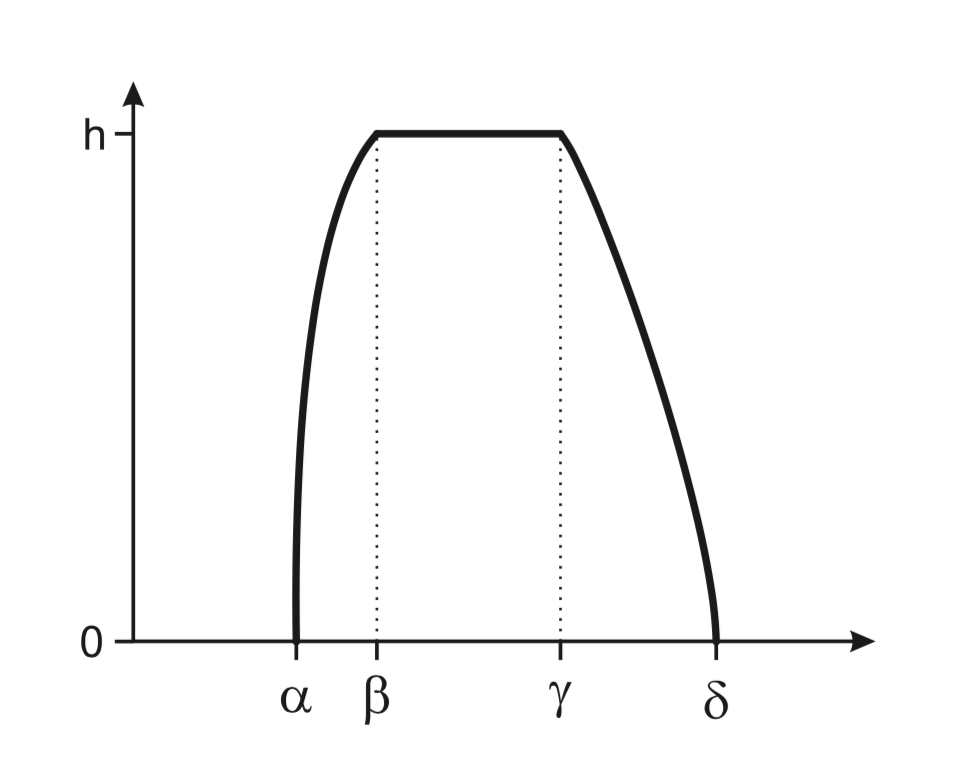
\includegraphics[width=0.9\textwidth]{gfx/fuzzynumber.png}
  \caption{\label{fig:generaltrapezoid}Número difuso generalizado.}
\end{figure}

Los números difusos que nos interesan a nosotros especialmente, y que utilizaremos para dar nuestra solución, son aquellos en los que las funciones $r$ y $s$ son lineales. Estos son llamados los \textbf{trapezoides}, veáse figura \ref{fig:trapezoid}, y tienen la siguiente forma de pertenencia de número difuso.

\begin{equation}\label{trapezoidrepresentation}
    f(x) = \left\{ { \begin{array}{cc}
                    0 & x < \alpha \\ 
                    h + \frac{(x-\beta)h}{\beta-\alpha} & x\in [\alpha,\beta) \\
                    h & x\in [\beta,\gamma] \\
                    h + \frac{(x-\gamma)h}{\delta-\gamma} & x\in (\gamma,\delta] \\
                    0 & x > \delta \\ 
                    \end{array}  } \right.
\end{equation}

\begin{figure}[h]
  \centering
  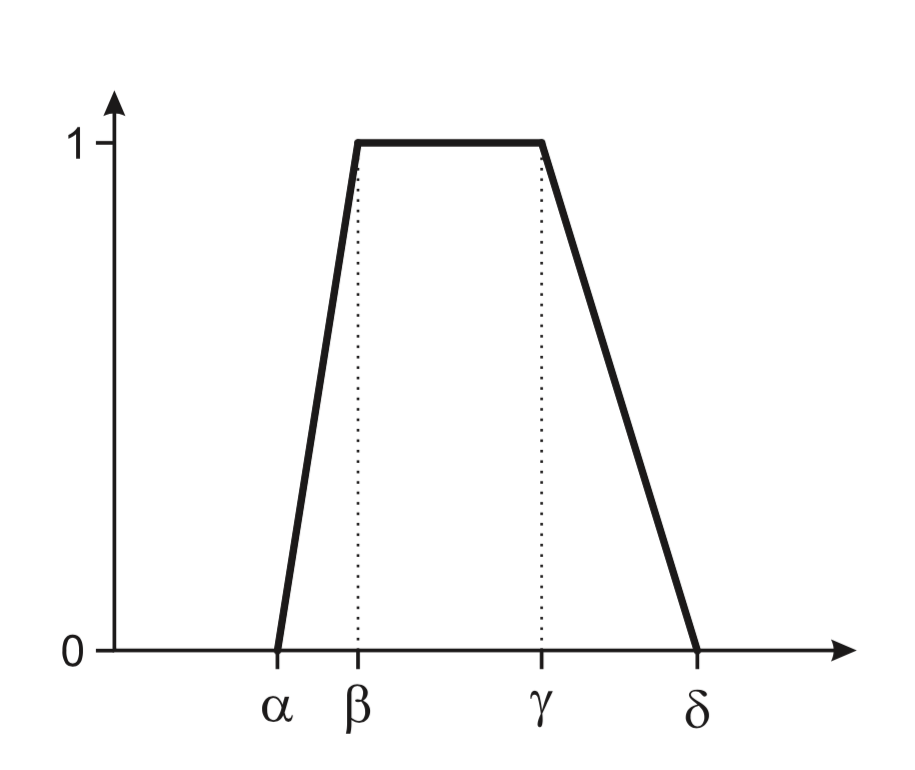
\includegraphics[width=0.9\textwidth]{gfx/trapezoid.png}
  \caption{\label{fig:trapezoid}Número difuso trapezoidal.}
\end{figure}

Además, habitualmente estará normalizado ($h=1$) y por tanto nos basta con una tupla $(\alpha, \beta, \gamma, \delta)$ para definir un número difuso.

\begin{remark}\label{notaciontrapezoide}
Notemos que esta representación nos vale incluso cuando se tengan solo 1,2 ó 3 valores. Estos serán llamados \textit{crisp}, \textit{intervalo} y \textit{triangulares} respectivamente. Con un valor $a$, tendremos $\alpha = \beta = \gamma = \delta = a$, con dos valores, $a,b$ tendremos $\alpha = \beta = a$ y $\gamma = \delta = b$ y con tres valores, $a,b,c$ tendremos $\beta = \gamma = b$. Veáse un ejemplo de ello para el caso triangular en \ref{fig:trapezoid3}
\end{remark}

\begin{figure}[h]
  \centering
  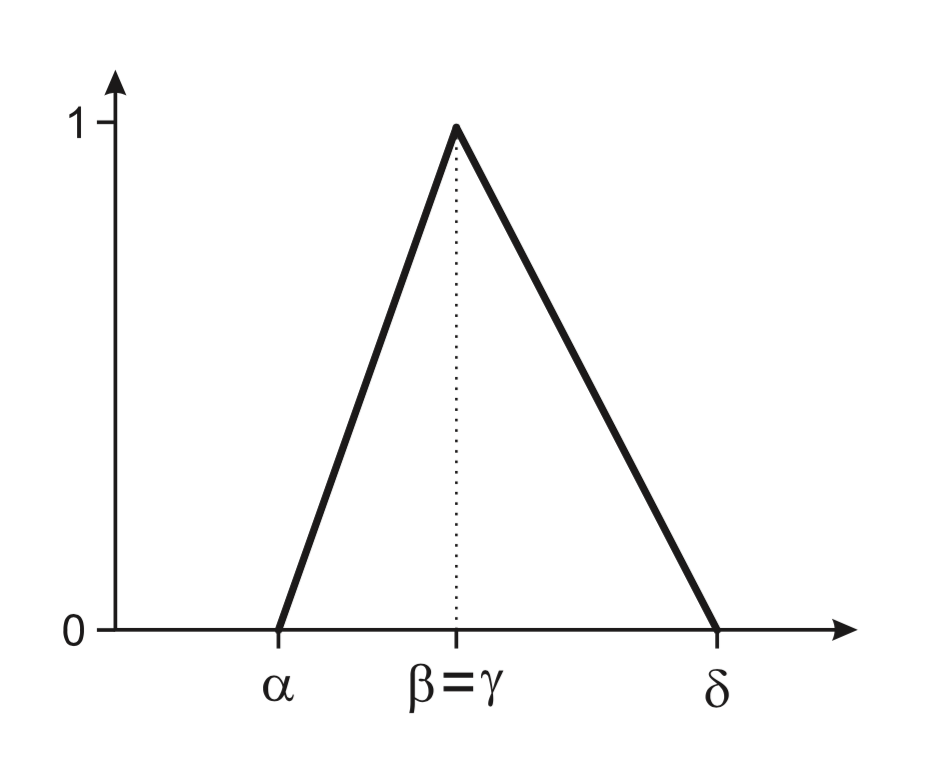
\includegraphics[width=0.9\textwidth]{gfx/trapezoid3.png}
  \caption{\label{fig:trapezoid3}Trapezoide con 3 valores.}
\end{figure}

\section{Información Imprecisa en bases de datos}

Vamos a introducir los precedentes existentes en el área de representación y tratamiento de información imprecisa en bases de datos. Se pueden encontrar referencias de un amplio abanico para dar solución al desafío que nos enfrentamos.

Además, el término ``imprecisa'', referida a la información, engloba varios significados que podemos distinguir \cite{fuzzynotion}:

\begin{itemize}
    \item Incompletitud: Información incompleta, es decir, no tenemos toda la información posible.
    \item Incertidumbre: No se sabe si la información es cierta o no.
    \item Desconocimiento: No se tiene información.
    \item Inaplicabilidad: La información de la que se dispone no es aplicable a ninguna entidad.
\end{itemize}

Podemos clasificar los distintos tipos de modelos en dos categorías según el uso o no de la lógica difusa. Dentro de las propuestas que utilizan lógica difusa, nos centraremos en el modelo GEFRED, en el que nos hemos basado para realizar la propuesta sobre MongoDB. Podemos obtener una visión conjunta de todas las propuestas que se van a mencionar a lo largo de esta sección en \cite{tesismedina, tesisbarranco, tesispepe}.

\subsection{Aproximaciones sin emplear lógica difusa}

Vamos a resumir las distintas propuestas que se han realizado sin utilizar la teoría de conjuntos difusos vista en este mismo capítulo, agrupadas por la técnica utilizada para llevar a cabo el propósito:

\begin{itemize}
    \item \textbf{Valores nulos}: E. Codd realizó la primera propuesta en \cite{codd} y fue evolucionándola en \cite{codd1, codd2, codd3}. Consiste en utilizar el valor \texttt{NULL} en todo el dominio disponible de la base de datos. Este valor indicaba que no se conocía el valor del atributo.
    \item \textbf{Valores por defecto}: Esta propuesta, publicada en \cite{date} surge por la idea del autor de que los valores nulos no habían sido tratados correctamente, y propone sustituirlos por un valor por defecto del dominio. Así, en caso de no conocer la información de un atributo, se asignaría el valor por defecto seleccionado para dicho atributo.
    \item \textbf{Rangos de valores}: Propuesta realizada por Grant en \cite{grant}, realizó una extensión del modelo relacional para almacenar un rango de valores posibles y la redefinición de los operadores para que en su evaluación se pudiese obtener el rango de valores \textit{verdadero}, \textit{falso} y \textit{quizás}.
     \item \textbf{Bases de datos estadísticas y probabilísticas}: En \cite{wong} se da una propuesta de bases de datos estadísticas, esto es, cada consulta resuelve la incertidumbre como un experimento estadístico obtiendo como resultado la tupla que minimice el error estadístico. En \cite{dbprobabilistic} se obtiene una propuesta para base de datos probabilística, asociando probabilidades a los valores de los atributos tratando a cada atributo como una distribución de probabilidad discreta.
\end{itemize}

\subsection{Bases de datos difusas}

Veamos ahora las propuestas que se han realizado para bases de datos utilizando la lógica difusa y teoría de conjuntos difusos. Estas propuestas se centran en añadir a cada tupla un \textit{grado}, normalmente en el intervalo $[0,1]$, a cada tupla.

Las distintas propuestas son las dadas por Buckles y Petry en \cite{buckles, buckles2, buckles3} basado en el concepto de relación de similitud, Prade y Testemale en \cite{prade, prade2, prade3, prade4} basada en la teoría de posibilidad, Umano y Fukami en \cite{fukami, fukami2, fukami3, fukami4} basado también en la teoría de la posibilidad, el modelo propuesto por Zemankova y Kaendel en \cite{zemankova, zemankova2} que realiza una representación imperfecta similar a los modelos posibilísticos, pero que adicionalmente desarrolla un lenguaje de manipulación de datos que analiza las relaciones entre posibilidad y certeza. Por último, la propuesta de Medina, Pons y Vila \cite{gefred}, el modelo GEFRED, que pretende unificar todas las propuestas anteriores y dar una solución completa al tratamiento de información imprecisa en base de datos relacional, se basa en lo que llaman \textit{Dominio difuso generalizado} y \textit{relación difusa generalizada}, a través de los cuales, GEFRED redefine los operadores del algebra relacional en el llamado \textit{Álgebra relacional difuso generalizado}. No entramos en detalle de estos operadores pues se trata de lenguaje SQL que no utilizaremos en este trabajo, pero puede verse en \cite{gefred}.

\subsection{Operadores difusos}\label{cdeg}

Para el tratamiento de información difusa, es necesario definir ciertos operadores para poder ejecutar consultas sobre la base de datos. En esta sección veremos los operadores que hemos utilizado para trabajar con esta información y el cómo obtener cada uno de ellos.

Cuando queremos comparar dos atributos difusos de una base de datos, dotamos a los valores de un grado de cumplimiento, al que llamaremos \textbf{cdeg}. Este grado de depende de la medida que estemos utilizando, en nuestro caso, vamos a considerar dos medidas distintas, las que llamaremos como medida de \textit{necesidad} y medida de \textit{posibilidad}.

\subsubsection{Operadores de igualdad difusos}

Sean $A$ y $B$ dos distribuciones de posibilidad trapezoidales, y sean $f_A$ y $f_B$ sus funciones de pertenencia, respectivamente, definidas sobre un dominio ordenado $\Omega$. Para calcular el grado de igualdad dependiendo de la medida, utilizamos las siguientes definiciones \cite{tesispepe}:

\begin{definition}[Operador FEQ]
Para comparar ambas distribuciones y obtener el grado de compatibilidad entre ellas, esto es, en qué medida son \texttt{posiblemente} iguales, se usa la ecuación:

\begin{equation}
    feq(A,B) = \sup_{x \in \Omega} \min (f_A(x), f_B(x))
\end{equation}
\end{definition}

\begin{definition}[Operador NFEQ]
Para comparar ambas distribuciones y obtener el grado de compatibilidad entre ellas, esto es, en qué medida son \texttt{necesariamente} iguales, se usa la ecuación:

\begin{equation}
    nfeq(A,B) = \inf_{x \in \Omega} \max (1-f_A(x), f_B(x))
\end{equation}
\end{definition}


\subsubsection{Operadores relacionales difusos}

Sean $A$ y $B$ dos distribuciones de posibilidad trapezoidales definidas sobre un dominio ordenado $\Omega$, con $A = \trapezoidA$ y $B=\trapezoidB$. Para calcular el grado de relación dependiendo de la medida, utilizamos las siguientes definiciones \cite{tesispepe}:

\begin{definition}[Operador FGT]
Para obtener el grado en que $A$ es \texttt{posiblemente} mayor que $B$, se usa la ecuación:

\begin{equation}
    fgt(A,B) = \left\{ { \begin{array}{ll}
                    1 & \text{si}\, \gamma_A \geq \delta_B \\ 
                    \frac{\delta_A - \gamma_B}{(\delta_B - \gamma_B)-(\gamma_A - \delta_A)} & \text{si}\, \gamma_A < \delta_B \, \text{y} \, \delta_A > \gamma_B \\
                    0 & \text{en otro caso} \\ 
                    \end{array}  } \right.
\end{equation}
\end{definition}

\begin{definition}[Operador NFGT]
Para obtener el grado en que $A$ es \texttt{necesariamente} mayor que $B$, se usa la ecuación:

\begin{equation}
    nfgt(A,B) = \left\{ { \begin{array}{ll}
                    1 & \text{si}\, \alpha_A \geq \delta_B \\ 
                    \frac{\beta_A - \gamma_B}{(\delta_B - \gamma_B)-(\alpha_A - \beta_A)} & \text{si}\, \alpha_A < \delta_B \, \text{y} \, \beta_A > \gamma_B \\
                    0 & \text{en otro caso} \\ 
                    \end{array}  } \right.
\end{equation}
\end{definition}

\begin{definition}[Operador FGTE]
Para obtener el grado en que $A$ es \texttt{posiblemente} mayor o igual que $B$, se usa la ecuación:

\begin{equation}
    fgte(A,B) = \left\{ { \begin{array}{ll}
                    1 & \text{si}\, \gamma_A \geq \beta_B \\ 
                    \frac{\delta_A - \alpha_B}{(\beta_B - \alpha_B)-(\gamma_A - \delta_A)} & \text{si}\, \gamma_A < \beta_B \, \text{y} \, \delta_A > \alpha_B \\
                    0 & \text{en otro caso} \\ 
                    \end{array}  } \right.
\end{equation}
\end{definition}

\begin{definition}[Operador NFGTE]
Para obtener el grado en que $A$ es \texttt{necesariamente} mayor o igual que $B$, se usa la ecuación:

\begin{equation}
    nfgte(A,B) = \left\{ { \begin{array}{ll}
                    1 & \text{si}\, \alpha_A \geq \beta_B \\ 
                    \frac{\beta_A - \alpha_B}{(\beta_B - \alpha_B)-(\alpha_A - \beta_A)} & \text{si}\, \alpha_A < \beta_B \, \text{y} \, \beta_A > \alpha_B \\
                    0 & \text{en otro caso} \\ 
                    \end{array}  } \right.
\end{equation}
\end{definition}

\begin{definition}[Operador FLT]
Para obtener el grado en que $A$ es \texttt{posiblemente} menor que $B$, se usa la ecuación:

\begin{equation}
    flt(A,B) = \left\{ { \begin{array}{ll}
                    1 & \text{si}\, \beta_A \leq \alpha_B \\ 
                    \frac{\alpha_A - \beta_B}{(\alpha_B - \beta_B)-(\beta_A - \alpha_A)} & \text{si}\, \beta_A > \alpha_B \, \text{y} \, \alpha_A < \beta_B \\
                    0 & \text{en otro caso} \\ 
                    \end{array}  } \right.
\end{equation}
\end{definition}

\begin{definition}[Operador NFLT]
Para obtener el grado en que $A$ es \texttt{necesariamente} menor que $B$, se usa la ecuación:

\begin{equation}
    nflt(A,B) = \left\{ { \begin{array}{ll}
                    1 & \text{si}\, \delta_A \leq \alpha_B \\ 
                    \frac{\gamma_A - \beta_B}{(\alpha_B - \beta_B)-(\delta_A - \gamma_A)} & \text{si}\, \delta_A > \alpha_B \, \text{y} \, \gamma_A < \beta_B \\
                    0 & \text{en otro caso} \\ 
                    \end{array}  } \right.
\end{equation}
\end{definition}

\begin{definition}[Operador FLTE]
Para obtener el grado en que $A$ es \texttt{posiblemente} menor o igual que $B$, se usa la ecuación:

\begin{equation}
    flte(A,B) = \left\{ { \begin{array}{ll}
                    1 & \text{si}\, \beta_A \leq \gamma_B \\ 
                    \frac{\delta_B - \alpha_A}{(\beta_A-\alpha_A)-(\gamma_B - \delta_B)} & \text{si}\, \beta_A > \gamma_B \, \text{y} \, \alpha_A < \delta_B \\
                    0 & \text{en otro caso} \\ 
                    \end{array}  } \right.
\end{equation}
\end{definition}

\begin{definition}[Operador NFLTE]
Para obtener el grado en que $A$ es \texttt{necesariamente} menor o igual que $B$, se usa la ecuación:

\begin{equation}
    nflte(A,B) = \left\{ { \begin{array}{ll}
                    1 & \text{si}\, \delta_A \leq \gamma_B \\ 
                    \frac{\gamma_A - \delta_B}{(\gamma_B - \delta_B)-(\delta_A - \gamma_A)} & \text{si}\, \delta_A > \gamma_B \, \text{y} \, \gamma_A < \delta_B \\
                    0 & \text{en otro caso} \\ 
                    \end{array}  } \right.
\end{equation}
\end{definition}

Una representación visual de lo que implica cada uno de estos operadores, puede verse en \cite[p.~172]{tesispepe}.
